\graphicspath{{img/ch3}}

\section{Thermal Characteristics}

\subsection{Thermal Stability and Anomalies}

The thermal environment within lunar pits provides a stark contrast to the extreme temperature fluctuations of the lunar surface. Data collected from the Diviner Lunar Radiometer Experiment reveal that the interior of pits maintains remarkably stable temperatures, with values ranging from approximately 250 to 290 K in permanently shadowed regions, even during the lunar night \cite{thermal-lunar-pits}. This is in contrast to the lunar surface, where temperatures vary dramatically between $\sim$100 K during the night and $\sim$400 K in direct sunlight due to the Moon’s lack of atmosphere.

\begin{figure}[H]
    \centering
    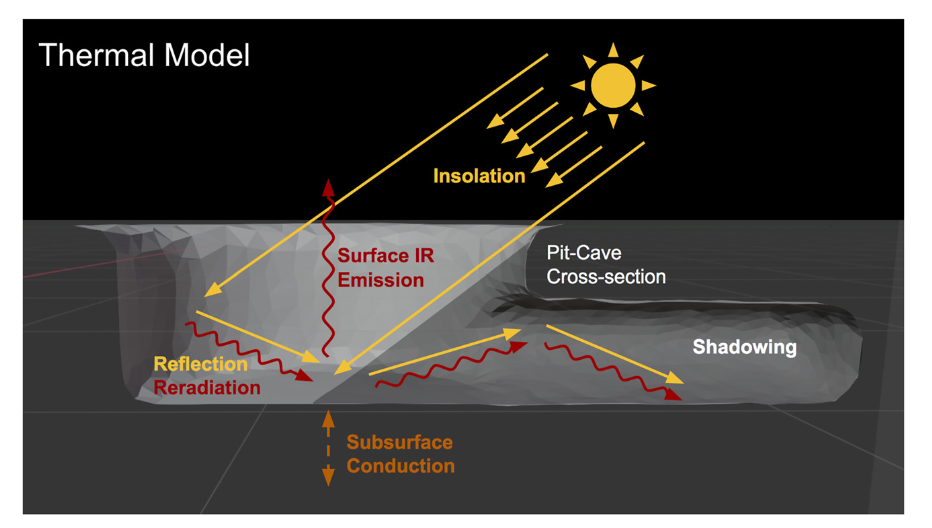
\includegraphics[width=0.6\linewidth]{lunar-pit-thermal-model.png}
    \caption{Schematic representation of heat transfer in lunar pits, illustrating shadowing, infrared emission, and subsurface conduction \cite{thermal-lunar-pits}.}
    \label{fig:lunar-pit-thermal-model}
\end{figure}

The thermal stability observed in pits results primarily from their geometry. Overhanging walls and limited sky exposure block direct solar radiation and mitigate radiative heat loss during the lunar night. As modeled by Horvath et al. \cite{thermal-lunar-pits}, this creates natural “blackbody cavities,” where incoming solar radiation is absorbed and redistributed internally. The floors of pits, such as those in Mare Tranquillitatis and Mare Ingenii, have been observed to remain up to 100 K warmer than the surrounding surface at night, confirming their thermal insulating properties \cite{thermal-lunar-pits, newer-thermal}.

\begin{figure}[H]
    \centering
    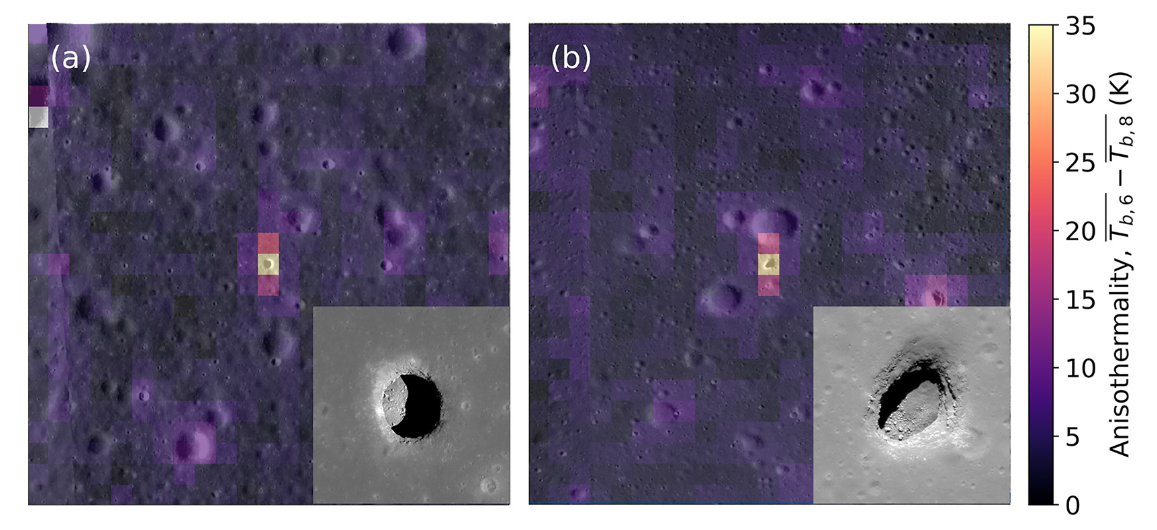
\includegraphics[width=0.7\linewidth]{lunar-pits-temperature-LROC.png}
    \caption{Temperature maps of Mare Tranquillitatis (a) and Mare Ingenii pits (b) measured by Diviner. Insets show NAC images for reference. Warm anomalies appear in pit interiors compared to surrounding surfaces \cite{thermal-lunar-pits}.}
    \label{fig:lunar-pits-temperatures-LROC}
\end{figure}

\subsection{Thermal Dynamics and Material Effects}

The thermal behavior of pit floors and walls is strongly influenced by their material composition. Numerical models comparing regolith-dominated and rock-dominated surfaces reveal key differences in diurnal temperature variations. Rock surfaces exhibit smaller temperature fluctuations due to their higher thermal conductivity, which allows for more efficient heat transfer and rapid equilibration. In contrast, regolith-covered surfaces show larger diurnal variations, as the insulating properties of lunar soil slow heat exchange, leading to higher daytime peaks and lower nighttime minima \cite{thermal-lunar-pits, newer-thermal}.

\begin{figure}[H]
    \centering
    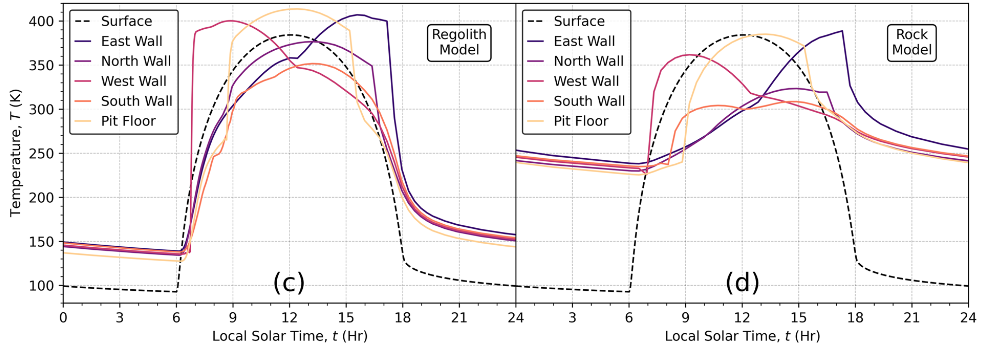
\includegraphics[width=0.9\linewidth]{lunar-pit-regolith-vs-stone-thermal.png}
    \caption{Simulated temperature profiles for lunar pits assuming regolith (c) and solid rock (d) floors. Rock surfaces show smaller diurnal variations due to higher thermal conductivity, while regolith exhibits greater fluctuations \cite{thermal-lunar-pits}.}
    \label{fig:regolith-vs-stone-thermal}
\end{figure}

This behavior has important implications for thermal stability. Pits with rocky floors maintain temperatures closer to equilibrium values due to their ability to distribute absorbed heat efficiently. Conversely, regolith-covered floors experience more pronounced temperature extremes, as their insulating nature restricts heat dissipation. These findings provide insights into the expected thermal environment within pits and can guide the selection of potential exploration and habitation sites.

\begin{figure}[H]
    \centering
    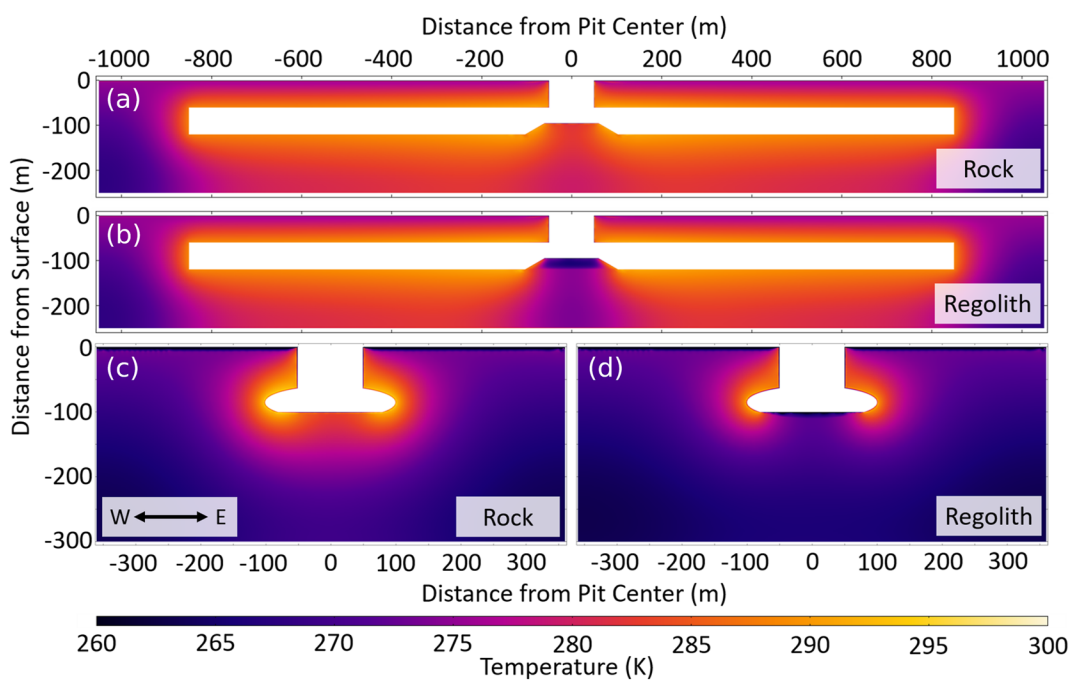
\includegraphics[width=0.75\linewidth]{thermal-simulation-lunar-pits-2d-regolith-rock.png}
    \caption{Equilibrium temperature distributions for rock (a, c) and regolith (b, d) surfaces in lunar pits and caves. The top row shows extended horizontal caves, while the bottom row focuses on vertical pits. Regolith surfaces (b, d) retain heat closer to the opening, while rock surfaces (a, c) exhibit cooler and more uniform internal temperatures \cite{thermal-lunar-pits}.}
    \label{fig:lunar-pit-equilibrium-temps}
\end{figure}


\subsection{Volatile Stability and Cold Traps}

Lunar pits have also been proposed as potential cold traps for volatiles, such as water ice, particularly in high-latitude regions. However, recent studies indicate that the enclosed geometry of pits leads to multiple scattering of infrared radiation, which raises internal temperatures and reduces their efficiency as cold traps compared to traditional craters \cite{newer-thermal}. Nevertheless, specific conditions—such as pits shadowed by exterior topography or connected to deeper caves—may still support the accumulation of volatiles \cite{newer-thermal, lunar-pits-numerical-modelling}.

Wilcoski et al. \cite{newer-thermal} demonstrate that volatile loss rates within pits are generally higher than in permanently shadowed regions (PSRs) of craters, making pits less efficient for long-term ice storage. However, their potential to provide protection from surface processes, such as micrometeoroid impacts and solar wind sputtering, remains an advantage for short-term volatile preservation.
